\documentclass[a4paper, 12pt]{article}

\usepackage[T1]{fontenc}
\usepackage[polish]{babel} 
\usepackage[utf8]{inputenc} 
\usepackage{indentfirst}
\let\lll\undefined
\usepackage{amssymb}
\usepackage{setspace}
\usepackage{fancyhdr}
\usepackage{graphicx} 

\pagestyle{fancy} 
\newcommand{\mainmatter}{\clearpage \cfoot{\thepage\ of \pageref{LastPage}}
\pagenumbering{arabic}}




\begin{document}
	\begin{titlepage}
		
		\begin{center}
    	\vspace{5cm}
    		\Large\textit{\textbf{SPRAWOZDANIE KOŃCOWE
    		\\''Gra w życie'' DLA JĘZYKA PROGRAMOWANIA C}}\\ 
		\vspace{15cm}
		\end{center} 

		\hfill\begin{minipage}{0.5\textwidth}
			\Large Wykonali:\newline
				1. Ivan Prakapets \newline
		\vspace{\baselineskip}
		\end{minipage}
	\end{titlepage}
\newpage
\mainmatter
\setlength{\headheight}{15pt}
\doublespacing
\tableofcontents
\newpage
	\section{Wprowadzone zmiany}
			\hspace*{1cm} W implementacji programu zaszły następujące zmiany względem złożeń specyfikacji implementacyjnej:
		\subsection{Moduł read$\_$and$\_$write$\_$png}
			\hspace*{1cm} Moduł \texttt{read$\_$and$\_$write$\_$png} składał się z trzech funkcji:
			\renewcommand{\labelitemi}{$\ast$}
		\begin{itemize}
			\item \texttt{void read$\_$png$\_$file ( char * )}
			\item \texttt{void write$\_$png$\_$file ( char * , int )}
			\item \texttt{void process$\_$file ( int ** )}
		\end{itemize}
			\hspace*{1cm} Została dodana funkcja: 
		\begin{itemize}
			\item \texttt{void process$\_$file$\_$for$\_$txt ( int ** )}
		\end{itemize}
			\hspace*{1cm} Funkcja process$\_$file$\_$for$\_$txt. Celem tej funkcji jest sprawdzanie pliku \texttt{txt} oraz wdrążenie funkcji \texttt{read$\_$png$\_$file} do gry.
			
		\subsection{Moduł read$\_$txt} 
			\hspace*{1cm} Moduł \texttt{read$\_$txt} nie został zmieniony.
\newpage
		\subsection{Moduł generacja}
			\hspace*{1cm} Moduł \texttt{generacja} składał się z dwóch funkcji: 
		\begin{itemize}
			\item \texttt{void print$\_$gen$\_$to$\_$file ( int ** )} 
			\item \texttt{void print$\_$gen ( int ** )} 
		\end{itemize}
			\hspace*{1cm} Została usunięta funkcja: 
		\begin{itemize}
			\item \texttt{void print$\_$gen ( int ** )} 
		\end{itemize}
			\hspace*{1cm} Celem usunięcia tej funkcji jest taka, że więciej jej nie potrzebowali.		
			
		\subsection{Moduł sasiadstwa}
			\hspace*{1cm} Moduł \texttt{sasiadstwa} składał się z dwóch funkcji z jednym imieniem 
		\begin{itemize}
			\item \texttt{int count$\_$neighbours ( int , int , int ** )} 
		\end{itemize}
			\hspace*{1cm} Została wprowadzona zmiana nazwy funkcji i dodana funkcja: 
		\begin{itemize}
			\item \texttt{int count$\_$neighbours$\_$Moore$\_$a ( int , int , int ** )}
			\item \texttt{int count$\_$neighbours$\_$Neumann ( int , int , int ** )}
		\end{itemize}
			\hspace*{1cm} To jest zrobiono dla ułatwienia programu, dlatego że musimy zrobić taki samy program w dwa różnych sposoby.
\newpage
	\section{Dodanie modułów}
			\hspace*{1cm} W implementacji programu zaszły następujące nowe moduły względem złożeń specyfikacji implementacyjnej:
		\subsection{Moduł regula$\_$generacji}
			\hspace*{1cm} Moduł \texttt{regula$\_$generacji} składa się z trzech funkcji:
		\begin{itemize}
			\item \texttt{int** create$\_$next$\_$gen$\_$Moore$\_$a ( int ** )} 
			\item \texttt{int** create$\_$next$\_$gen$\_$Neumann ( int ** )} 
			\item \texttt{void free$\_$matrix ( int ** )}
		\end{itemize}
		
		\begin{enumerate}
			\item Funkcja \texttt{create$\_$next$\_$gen$\_$Moore$\_$a}. 
			Celem tej funkcji jest stworzenie następującej generacji dla sąsiedztwa Moore$\_$a.
			\item Funkcja \texttt{create$\_$next$\_$gen$\_$Neumann}. 
			Celem tej funkcjii jest stworzenie następującej generacji dla sąsiedztwa Neumann.
			\item Funkcja \texttt{free$\_$matrix}. 
			Celem tej funkcji jest usunięcie wycieków pamięci (oczyszczenie tablicy matrix).
		\end{enumerate}

		\subsection{Moduł symulator}
			\hspace*{1cm} Moduł \texttt{symulator} składa się z 5 funkcji:
		\begin{itemize}
			\item \texttt{void symulator$\_$Moore$\_$a ( int , int ** , char* )}
			\item \texttt{void symulator$\_$Neumann ( int , int ** , char* )}
			\item \texttt{void symulator$\_$Moore$\_$a$\_$txt ( int , int ** , char* )}
			\item \texttt{void symulator$\_$Neumann$\_$txt ( int , int ** , char* )}
			\item \texttt{void usage ()}
		\end{itemize}
		
		\begin{enumerate}
			\item Funkcja \texttt{symulator$\_$Moore$\_$a}. 
			Celem tej funkcji jest symulacja dla sąsiedztwa Moore$\_$a.
			\item Funkcja \texttt{symulator$\_$Neumann}. 
			Celem tej funkcji jest symulacja dla sąsiedztwa Neumann.
			\item Funkcja \texttt{symulator$\_$Moore$\_$a$\_$txt}. 
			Celem tej funkcji jest symulacja dla sąsiedztwa Moore$\_$ w formacie \texttt{.txt}.
			\item Funkcja \texttt{symulator$\_$Neumann$\_$txt}. 
			Celem tej funkcji jest symulacja dla sąsiedztwa Neumann w formacie \texttt{.txt}.
			\item Funkcja \texttt{usage}. 
			Celem tej funkcji jest wyświetlenie informacji jak uruchomić i korzystać z programu.
		\end{enumerate}
		
		\subsection{Moduł test$\_$game}
			\hspace*{1cm} Moduł \texttt{test$\_$game} składa się z jednej testującej funkcji:
		\begin{itemize}
			\item \texttt{int main ( int , char * )}
		\end{itemize}		 
		która sprawdza poprawne wczytywanie z pliku \texttt{.txt} i z pliku \texttt{.png} również wypisuję błędy.
\newpage
	\section{Działania i wyniki programu}
			\hspace*{1cm} Po napisaniu koda są takie wyniki:
		\subsection{Kompilacja i uruchomienie}
			\subsubsection{Kompilacja}
			\hspace*{1cm} Ekran działania programu:
		\begin{figure}[h]
			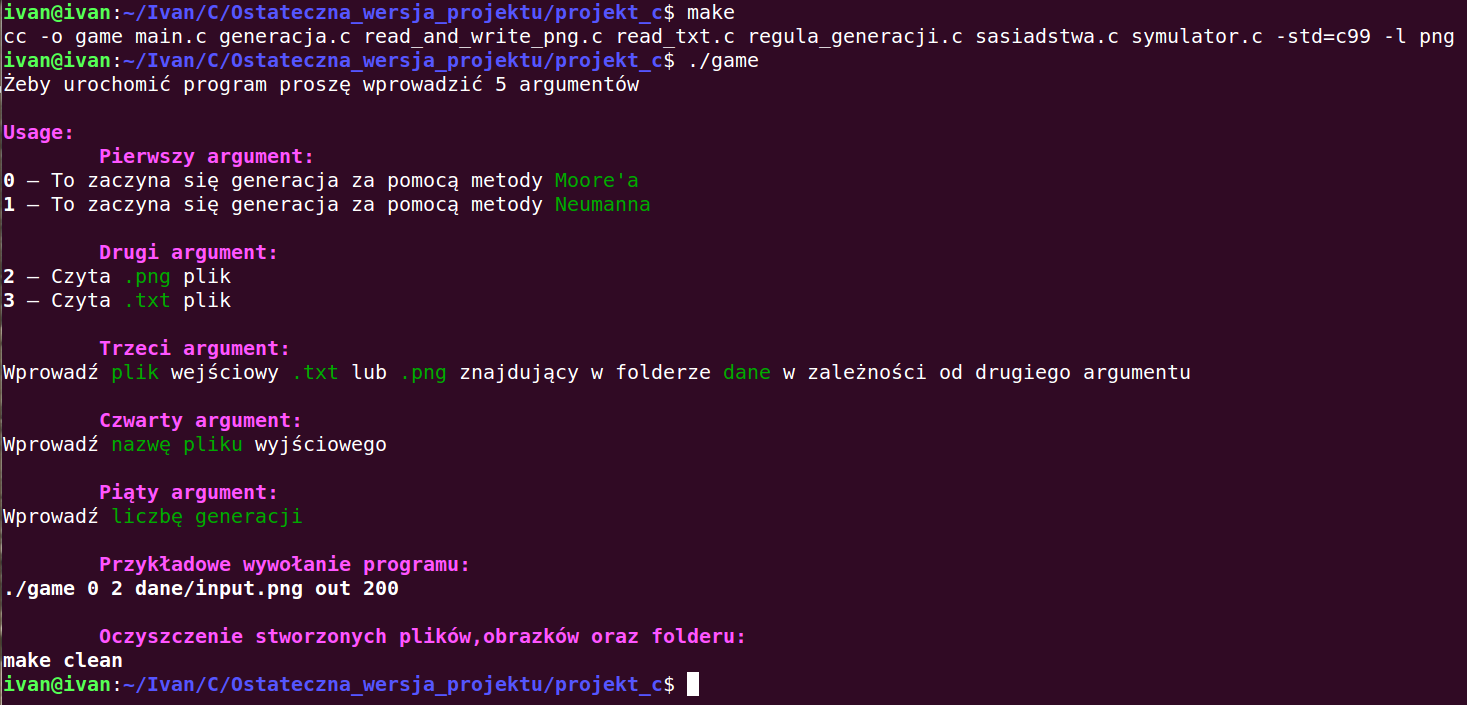
\includegraphics[width=\textwidth]{ekran.png}
			\caption{Ekran programu}
		\end{figure}	
			\subsubsection{Uruchomienie}
			\hspace*{1cm} Przykładowa komenda dla uruchomienia:
		\begin{figure}[h]
			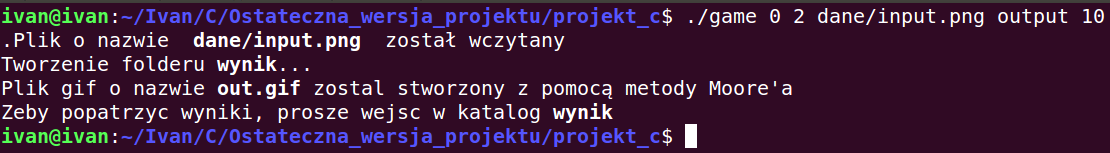
\includegraphics[width=\textwidth]{komenda_uruchomienia.png}
			\caption{Przykład komendy}
		\end{figure}	
\newpage
		\subsection{Wyniki programu}
			\subsubsection{Działania  programu dla plików \texttt{.png}}
			\hspace*{1cm} Plik wejściowego \texttt{dane/input.png} ma postać:
		\begin{figure}[h]
			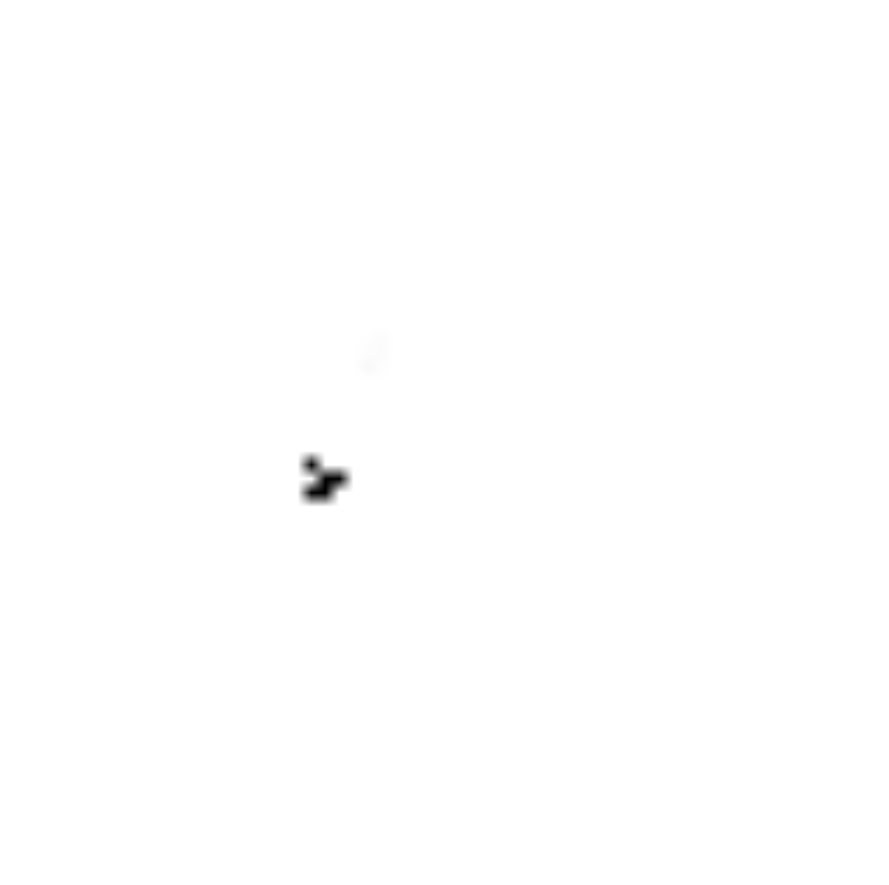
\includegraphics[width=\textwidth]{plik_wejsciowy_png.png}
			\caption{Plik wejściowy \texttt{input.png}}
		\end{figure}
\newpage
			\hspace*{1cm} Plik końcowy numer 116 \texttt{wynik/output$\_$116.png} ma postać:
		\begin{figure}[h]
			
\includegraphics[width=\textwidth]{plik_koncowy_png.png}
			\caption{Plik końcowy \texttt{output$\_$116.png}}
		\end{figure}
\newpage
			\subsubsection{Działania programu dla plików \texttt{.txt}}
			\hspace*{1cm} Plik wejściowy ma postać:
		\begin{figure}[h]
			
\includegraphics[width=\textwidth]{plik_wejsciowy_txt.png}
			\caption{Plik wejściowy}
		\end{figure}
\newpage
			\hspace*{1cm} Plik końcowy ma postać:
		\begin{figure}[h]
			
\includegraphics[width=\textwidth]{plik_koncowy_txt.png}
			\caption{Plik końcowy \texttt{wynik$\_$116.txt}}
		\end{figure}
\newpage
	\section{Wnioski}
			\hspace*{1cm} Podczas implementacji programu zaszło kilka zmian względem założeń ze specyfikacji implementacyjnej. Wynikały one głównie z lepszego rozeznania problemu, a także z zauważania oddzielnych i niezależnych funkcjonalności w większych funkcjach. Zostały też przeprowadzone zmiany kosmetyczne dotyczące nazw modułów i wygłądu programu, mające na celu wyeliminowanie nieścisłości kodu oraz poprawę jego czytelności. Wówczas podstawowe i najważniejsze założenia pochodzące ze specyfikacji implementacyjnej zostały zgodne z pierwotnymi ustaleniami, co potwierdza dobrze przemyślaną koncepcję systemu zawartą w specyfikacji funkcjonalnej oraz implementacyjnej. 
		

\label{LastPage}~
\label{LastPageOfBackMatter}~		
\end{document}